% Created by tikzDevice version 0.12 on 2019-02-27 16:44:06
% !TEX encoding = UTF-8 Unicode
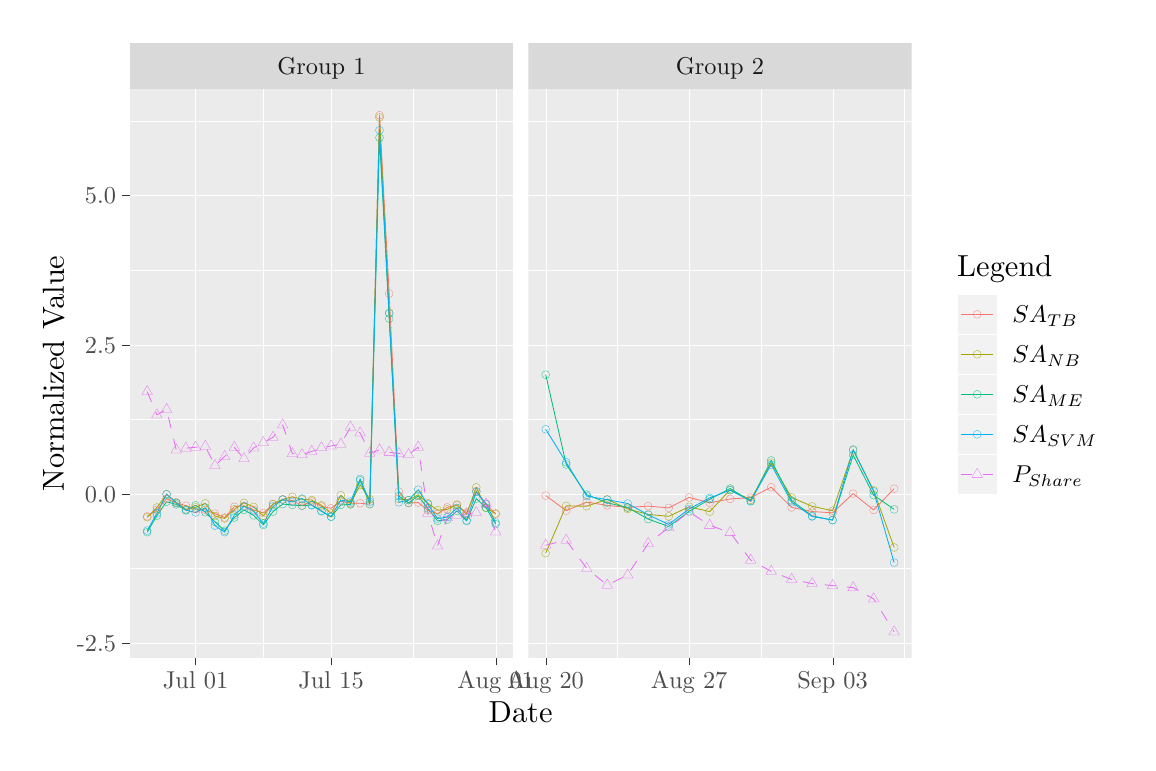
\begin{tikzpicture}[x=1pt,y=1pt]
\definecolor{fillColor}{RGB}{255,255,255}
\path[use as bounding box,fill=fillColor,fill opacity=0.00] (0,0) rectangle (397.48,258.37);
\begin{scope}
\path[clip] (  0.00,  0.00) rectangle (397.48,258.37);
\definecolor{drawColor}{RGB}{255,255,255}
\definecolor{fillColor}{RGB}{255,255,255}

\path[draw=drawColor,line width= 0.1pt,line join=round,line cap=round,fill=fillColor] (  0.00, -0.00) rectangle (397.48,258.37);
\end{scope}
\begin{scope}
\path[clip] ( 36.90, 30.73) rectangle (175.39,236.06);
\definecolor{fillColor}{gray}{0.92}

\path[fill=fillColor] ( 36.90, 30.73) rectangle (175.39,236.06);
\definecolor{drawColor}{RGB}{255,255,255}

\path[draw=drawColor,line width= 0.1pt,line join=round] ( 36.90, 62.94) --
	(175.39, 62.94);

\path[draw=drawColor,line width= 0.1pt,line join=round] ( 36.90,116.85) --
	(175.39,116.85);

\path[draw=drawColor,line width= 0.1pt,line join=round] ( 36.90,170.76) --
	(175.39,170.76);

\path[draw=drawColor,line width= 0.1pt,line join=round] ( 36.90,224.68) --
	(175.39,224.68);

\path[draw=drawColor,line width= 0.1pt,line join=round] ( 85.16, 30.73) --
	( 85.16,236.06);

\path[draw=drawColor,line width= 0.1pt,line join=round] (139.37, 30.73) --
	(139.37,236.06);

\path[draw=drawColor,line width= 0.1pt,line join=round] ( 36.90, 35.99) --
	(175.39, 35.99);

\path[draw=drawColor,line width= 0.1pt,line join=round] ( 36.90, 89.90) --
	(175.39, 89.90);

\path[draw=drawColor,line width= 0.1pt,line join=round] ( 36.90,143.81) --
	(175.39,143.81);

\path[draw=drawColor,line width= 0.1pt,line join=round] ( 36.90,197.72) --
	(175.39,197.72);

\path[draw=drawColor,line width= 0.1pt,line join=round] ( 60.68, 30.73) --
	( 60.68,236.06);

\path[draw=drawColor,line width= 0.1pt,line join=round] (109.64, 30.73) --
	(109.64,236.06);

\path[draw=drawColor,line width= 0.1pt,line join=round] (169.10, 30.73) --
	(169.10,236.06);
\definecolor{drawColor}{RGB}{248,118,109}

\path[draw=drawColor,line width= 0.3pt,line join=round] ( 43.20, 81.79) --
	( 46.69, 84.10) --
	( 50.19, 88.13) --
	( 53.69, 86.63) --
	( 57.18, 85.65) --
	( 60.68, 84.36) --
	( 64.18, 84.10) --
	( 67.68, 82.76) --
	( 71.17, 81.37) --
	( 74.67, 85.25) --
	( 78.17, 85.59) --
	( 81.67, 84.11) --
	( 85.16, 82.99) --
	( 88.66, 86.17) --
	( 92.16, 87.87) --
	( 95.65, 87.51) --
	( 99.15, 85.74) --
	(102.65, 87.16) --
	(106.15, 85.38) --
	(109.64, 84.69) --
	(113.14, 87.29) --
	(116.64, 86.55) --
	(120.14, 86.52) --
	(123.63, 86.20) --
	(127.13,226.73) --
	(130.63,162.31) --
	(134.13, 90.71) --
	(137.62, 86.64) --
	(141.12, 86.77) --
	(144.62, 83.97) --
	(148.11, 82.74) --
	(151.61, 85.02) --
	(155.11, 85.83) --
	(158.61, 83.10) --
	(162.10, 90.95) --
	(165.60, 86.36) --
	(169.10, 82.56);
\definecolor{drawColor}{RGB}{163,165,0}

\path[draw=drawColor,line width= 0.3pt,line join=round] ( 43.20, 81.47) --
	( 46.69, 84.97) --
	( 50.19, 89.75) --
	( 53.69, 86.84) --
	( 57.18, 84.35) --
	( 60.68, 85.05) --
	( 64.18, 86.49) --
	( 67.68, 81.90) --
	( 71.17, 81.02) --
	( 74.67, 84.33) --
	( 78.17, 86.66) --
	( 81.67, 85.19) --
	( 85.16, 81.98) --
	( 88.66, 86.27) --
	( 92.16, 87.94) --
	( 95.65, 88.83) --
	( 99.15, 87.94) --
	(102.65, 87.67) --
	(106.15, 85.77) --
	(109.64, 82.85) --
	(113.14, 89.44) --
	(116.64, 86.37) --
	(120.14, 93.12) --
	(123.63, 87.97) --
	(127.13,225.91) --
	(130.63,155.35) --
	(134.13, 88.12) --
	(137.62, 87.62) --
	(141.12, 89.60) --
	(144.62, 86.51) --
	(148.11, 84.02) --
	(151.61, 84.30) --
	(155.11, 86.01) --
	(158.61, 82.48) --
	(162.10, 92.29) --
	(165.60, 84.85) --
	(169.10, 82.84);
\definecolor{drawColor}{RGB}{0,191,125}

\path[draw=drawColor,line width= 0.3pt,line join=round] ( 43.20, 76.06) --
	( 46.69, 82.03) --
	( 50.19, 87.08) --
	( 53.69, 86.09) --
	( 57.18, 83.95) --
	( 60.68, 85.79) --
	( 64.18, 83.28) --
	( 67.68, 79.79) --
	( 71.17, 76.59) --
	( 74.67, 81.35) --
	( 78.17, 84.11) --
	( 81.67, 82.13) --
	( 85.16, 78.68) --
	( 88.66, 83.52) --
	( 92.16, 86.21) --
	( 95.65, 85.90) --
	( 99.15, 85.60) --
	(102.65, 85.93) --
	(106.15, 83.75) --
	(109.64, 81.60) --
	(113.14, 85.91) --
	(116.64, 86.09) --
	(120.14, 94.77) --
	(123.63, 86.21) --
	(127.13,218.60) --
	(130.63,153.23) --
	(134.13, 89.12) --
	(137.62, 86.64) --
	(141.12, 89.16) --
	(144.62, 84.63) --
	(148.11, 80.17) --
	(151.61, 80.61) --
	(155.11, 83.73) --
	(158.61, 80.11) --
	(162.10, 88.19) --
	(165.60, 84.95) --
	(169.10, 78.96);
\definecolor{drawColor}{RGB}{0,176,246}

\path[draw=drawColor,line width= 0.3pt,line join=round] ( 43.20, 76.64) --
	( 46.69, 82.90) --
	( 50.19, 89.82) --
	( 53.69, 86.63) --
	( 57.18, 84.03) --
	( 60.68, 83.18) --
	( 64.18, 84.89) --
	( 67.68, 78.43) --
	( 71.17, 76.07) --
	( 74.67, 82.23) --
	( 78.17, 85.39) --
	( 81.67, 83.61) --
	( 85.16, 79.19) --
	( 88.66, 85.37) --
	( 92.16, 87.83) --
	( 95.65, 86.98) --
	( 99.15, 88.23) --
	(102.65, 85.79) --
	(106.15, 83.61) --
	(109.64, 81.72) --
	(113.14, 87.67) --
	(116.64, 87.12) --
	(120.14, 95.33) --
	(123.63, 87.05) --
	(127.13,221.32) --
	(130.63,155.11) --
	(134.13, 86.87) --
	(137.62, 87.64) --
	(141.12, 91.42) --
	(144.62, 86.15) --
	(148.11, 80.96) --
	(151.61, 81.54) --
	(155.11, 84.88) --
	(158.61, 80.34) --
	(162.10, 90.67) --
	(165.60, 86.26) --
	(169.10, 79.55);
\definecolor{drawColor}{RGB}{231,107,243}

\path[draw=drawColor,line width= 0.3pt,dash pattern=on 4pt off 4pt ,line join=round] ( 43.20,126.85) --
	( 46.69,118.47) --
	( 50.19,120.44) --
	( 53.69,105.78) --
	( 57.18,106.43) --
	( 60.68,106.76) --
	( 64.18,107.09) --
	( 67.68,100.15) --
	( 71.17,103.42) --
	( 74.67,106.69) --
	( 78.17,102.63) --
	( 81.67,106.50) --
	( 85.16,108.43) --
	( 88.66,110.36) --
	( 92.16,114.81) --
	( 95.65,104.47) --
	( 99.15,104.07) --
	(102.65,105.25) --
	(106.15,106.56) --
	(109.64,107.22) --
	(113.14,107.87) --
	(116.64,114.02) --
	(120.14,111.93) --
	(123.63,104.60) --
	(127.13,105.78) --
	(130.63,104.93) --
	(134.13,104.50) --
	(137.62,104.07) --
	(141.12,106.82) --
	(144.62, 82.87) --
	(148.11, 71.09) --
	(151.61, 81.30) --
	(155.11, 82.21) --
	(158.61, 82.67) --
	(162.10, 83.13) --
	(165.60, 86.27) --
	(169.10, 76.19);
\definecolor{drawColor}{RGB}{248,118,109}

\path[draw=drawColor,line width= 0.1pt,line join=round,line cap=round] ( 43.20, 81.79) circle (  1.43);

\path[draw=drawColor,line width= 0.1pt,line join=round,line cap=round] ( 46.69, 84.10) circle (  1.43);

\path[draw=drawColor,line width= 0.1pt,line join=round,line cap=round] ( 50.19, 88.13) circle (  1.43);

\path[draw=drawColor,line width= 0.1pt,line join=round,line cap=round] ( 53.69, 86.63) circle (  1.43);

\path[draw=drawColor,line width= 0.1pt,line join=round,line cap=round] ( 57.18, 85.65) circle (  1.43);

\path[draw=drawColor,line width= 0.1pt,line join=round,line cap=round] ( 60.68, 84.36) circle (  1.43);

\path[draw=drawColor,line width= 0.1pt,line join=round,line cap=round] ( 64.18, 84.10) circle (  1.43);

\path[draw=drawColor,line width= 0.1pt,line join=round,line cap=round] ( 67.68, 82.76) circle (  1.43);

\path[draw=drawColor,line width= 0.1pt,line join=round,line cap=round] ( 71.17, 81.37) circle (  1.43);

\path[draw=drawColor,line width= 0.1pt,line join=round,line cap=round] ( 74.67, 85.25) circle (  1.43);

\path[draw=drawColor,line width= 0.1pt,line join=round,line cap=round] ( 78.17, 85.59) circle (  1.43);

\path[draw=drawColor,line width= 0.1pt,line join=round,line cap=round] ( 81.67, 84.11) circle (  1.43);

\path[draw=drawColor,line width= 0.1pt,line join=round,line cap=round] ( 85.16, 82.99) circle (  1.43);

\path[draw=drawColor,line width= 0.1pt,line join=round,line cap=round] ( 88.66, 86.17) circle (  1.43);

\path[draw=drawColor,line width= 0.1pt,line join=round,line cap=round] ( 92.16, 87.87) circle (  1.43);

\path[draw=drawColor,line width= 0.1pt,line join=round,line cap=round] ( 95.65, 87.51) circle (  1.43);

\path[draw=drawColor,line width= 0.1pt,line join=round,line cap=round] ( 99.15, 85.74) circle (  1.43);

\path[draw=drawColor,line width= 0.1pt,line join=round,line cap=round] (102.65, 87.16) circle (  1.43);

\path[draw=drawColor,line width= 0.1pt,line join=round,line cap=round] (106.15, 85.38) circle (  1.43);

\path[draw=drawColor,line width= 0.1pt,line join=round,line cap=round] (109.64, 84.69) circle (  1.43);

\path[draw=drawColor,line width= 0.1pt,line join=round,line cap=round] (113.14, 87.29) circle (  1.43);

\path[draw=drawColor,line width= 0.1pt,line join=round,line cap=round] (116.64, 86.55) circle (  1.43);

\path[draw=drawColor,line width= 0.1pt,line join=round,line cap=round] (120.14, 86.52) circle (  1.43);

\path[draw=drawColor,line width= 0.1pt,line join=round,line cap=round] (123.63, 86.20) circle (  1.43);

\path[draw=drawColor,line width= 0.1pt,line join=round,line cap=round] (127.13,226.73) circle (  1.43);

\path[draw=drawColor,line width= 0.1pt,line join=round,line cap=round] (130.63,162.31) circle (  1.43);

\path[draw=drawColor,line width= 0.1pt,line join=round,line cap=round] (134.13, 90.71) circle (  1.43);

\path[draw=drawColor,line width= 0.1pt,line join=round,line cap=round] (137.62, 86.64) circle (  1.43);

\path[draw=drawColor,line width= 0.1pt,line join=round,line cap=round] (141.12, 86.77) circle (  1.43);

\path[draw=drawColor,line width= 0.1pt,line join=round,line cap=round] (144.62, 83.97) circle (  1.43);

\path[draw=drawColor,line width= 0.1pt,line join=round,line cap=round] (148.11, 82.74) circle (  1.43);

\path[draw=drawColor,line width= 0.1pt,line join=round,line cap=round] (151.61, 85.02) circle (  1.43);

\path[draw=drawColor,line width= 0.1pt,line join=round,line cap=round] (155.11, 85.83) circle (  1.43);

\path[draw=drawColor,line width= 0.1pt,line join=round,line cap=round] (158.61, 83.10) circle (  1.43);

\path[draw=drawColor,line width= 0.1pt,line join=round,line cap=round] (162.10, 90.95) circle (  1.43);

\path[draw=drawColor,line width= 0.1pt,line join=round,line cap=round] (165.60, 86.36) circle (  1.43);

\path[draw=drawColor,line width= 0.1pt,line join=round,line cap=round] (169.10, 82.56) circle (  1.43);
\definecolor{drawColor}{RGB}{163,165,0}

\path[draw=drawColor,line width= 0.1pt,line join=round,line cap=round] ( 43.20, 81.47) circle (  1.43);

\path[draw=drawColor,line width= 0.1pt,line join=round,line cap=round] ( 46.69, 84.97) circle (  1.43);

\path[draw=drawColor,line width= 0.1pt,line join=round,line cap=round] ( 50.19, 89.75) circle (  1.43);

\path[draw=drawColor,line width= 0.1pt,line join=round,line cap=round] ( 53.69, 86.84) circle (  1.43);

\path[draw=drawColor,line width= 0.1pt,line join=round,line cap=round] ( 57.18, 84.35) circle (  1.43);

\path[draw=drawColor,line width= 0.1pt,line join=round,line cap=round] ( 60.68, 85.05) circle (  1.43);

\path[draw=drawColor,line width= 0.1pt,line join=round,line cap=round] ( 64.18, 86.49) circle (  1.43);

\path[draw=drawColor,line width= 0.1pt,line join=round,line cap=round] ( 67.68, 81.90) circle (  1.43);

\path[draw=drawColor,line width= 0.1pt,line join=round,line cap=round] ( 71.17, 81.02) circle (  1.43);

\path[draw=drawColor,line width= 0.1pt,line join=round,line cap=round] ( 74.67, 84.33) circle (  1.43);

\path[draw=drawColor,line width= 0.1pt,line join=round,line cap=round] ( 78.17, 86.66) circle (  1.43);

\path[draw=drawColor,line width= 0.1pt,line join=round,line cap=round] ( 81.67, 85.19) circle (  1.43);

\path[draw=drawColor,line width= 0.1pt,line join=round,line cap=round] ( 85.16, 81.98) circle (  1.43);

\path[draw=drawColor,line width= 0.1pt,line join=round,line cap=round] ( 88.66, 86.27) circle (  1.43);

\path[draw=drawColor,line width= 0.1pt,line join=round,line cap=round] ( 92.16, 87.94) circle (  1.43);

\path[draw=drawColor,line width= 0.1pt,line join=round,line cap=round] ( 95.65, 88.83) circle (  1.43);

\path[draw=drawColor,line width= 0.1pt,line join=round,line cap=round] ( 99.15, 87.94) circle (  1.43);

\path[draw=drawColor,line width= 0.1pt,line join=round,line cap=round] (102.65, 87.67) circle (  1.43);

\path[draw=drawColor,line width= 0.1pt,line join=round,line cap=round] (106.15, 85.77) circle (  1.43);

\path[draw=drawColor,line width= 0.1pt,line join=round,line cap=round] (109.64, 82.85) circle (  1.43);

\path[draw=drawColor,line width= 0.1pt,line join=round,line cap=round] (113.14, 89.44) circle (  1.43);

\path[draw=drawColor,line width= 0.1pt,line join=round,line cap=round] (116.64, 86.37) circle (  1.43);

\path[draw=drawColor,line width= 0.1pt,line join=round,line cap=round] (120.14, 93.12) circle (  1.43);

\path[draw=drawColor,line width= 0.1pt,line join=round,line cap=round] (123.63, 87.97) circle (  1.43);

\path[draw=drawColor,line width= 0.1pt,line join=round,line cap=round] (127.13,225.91) circle (  1.43);

\path[draw=drawColor,line width= 0.1pt,line join=round,line cap=round] (130.63,155.35) circle (  1.43);

\path[draw=drawColor,line width= 0.1pt,line join=round,line cap=round] (134.13, 88.12) circle (  1.43);

\path[draw=drawColor,line width= 0.1pt,line join=round,line cap=round] (137.62, 87.62) circle (  1.43);

\path[draw=drawColor,line width= 0.1pt,line join=round,line cap=round] (141.12, 89.60) circle (  1.43);

\path[draw=drawColor,line width= 0.1pt,line join=round,line cap=round] (144.62, 86.51) circle (  1.43);

\path[draw=drawColor,line width= 0.1pt,line join=round,line cap=round] (148.11, 84.02) circle (  1.43);

\path[draw=drawColor,line width= 0.1pt,line join=round,line cap=round] (151.61, 84.30) circle (  1.43);

\path[draw=drawColor,line width= 0.1pt,line join=round,line cap=round] (155.11, 86.01) circle (  1.43);

\path[draw=drawColor,line width= 0.1pt,line join=round,line cap=round] (158.61, 82.48) circle (  1.43);

\path[draw=drawColor,line width= 0.1pt,line join=round,line cap=round] (162.10, 92.29) circle (  1.43);

\path[draw=drawColor,line width= 0.1pt,line join=round,line cap=round] (165.60, 84.85) circle (  1.43);

\path[draw=drawColor,line width= 0.1pt,line join=round,line cap=round] (169.10, 82.84) circle (  1.43);
\definecolor{drawColor}{RGB}{0,191,125}

\path[draw=drawColor,line width= 0.1pt,line join=round,line cap=round] ( 43.20, 76.06) circle (  1.43);

\path[draw=drawColor,line width= 0.1pt,line join=round,line cap=round] ( 46.69, 82.03) circle (  1.43);

\path[draw=drawColor,line width= 0.1pt,line join=round,line cap=round] ( 50.19, 87.08) circle (  1.43);

\path[draw=drawColor,line width= 0.1pt,line join=round,line cap=round] ( 53.69, 86.09) circle (  1.43);

\path[draw=drawColor,line width= 0.1pt,line join=round,line cap=round] ( 57.18, 83.95) circle (  1.43);

\path[draw=drawColor,line width= 0.1pt,line join=round,line cap=round] ( 60.68, 85.79) circle (  1.43);

\path[draw=drawColor,line width= 0.1pt,line join=round,line cap=round] ( 64.18, 83.28) circle (  1.43);

\path[draw=drawColor,line width= 0.1pt,line join=round,line cap=round] ( 67.68, 79.79) circle (  1.43);

\path[draw=drawColor,line width= 0.1pt,line join=round,line cap=round] ( 71.17, 76.59) circle (  1.43);

\path[draw=drawColor,line width= 0.1pt,line join=round,line cap=round] ( 74.67, 81.35) circle (  1.43);

\path[draw=drawColor,line width= 0.1pt,line join=round,line cap=round] ( 78.17, 84.11) circle (  1.43);

\path[draw=drawColor,line width= 0.1pt,line join=round,line cap=round] ( 81.67, 82.13) circle (  1.43);

\path[draw=drawColor,line width= 0.1pt,line join=round,line cap=round] ( 85.16, 78.68) circle (  1.43);

\path[draw=drawColor,line width= 0.1pt,line join=round,line cap=round] ( 88.66, 83.52) circle (  1.43);

\path[draw=drawColor,line width= 0.1pt,line join=round,line cap=round] ( 92.16, 86.21) circle (  1.43);

\path[draw=drawColor,line width= 0.1pt,line join=round,line cap=round] ( 95.65, 85.90) circle (  1.43);

\path[draw=drawColor,line width= 0.1pt,line join=round,line cap=round] ( 99.15, 85.60) circle (  1.43);

\path[draw=drawColor,line width= 0.1pt,line join=round,line cap=round] (102.65, 85.93) circle (  1.43);

\path[draw=drawColor,line width= 0.1pt,line join=round,line cap=round] (106.15, 83.75) circle (  1.43);

\path[draw=drawColor,line width= 0.1pt,line join=round,line cap=round] (109.64, 81.60) circle (  1.43);

\path[draw=drawColor,line width= 0.1pt,line join=round,line cap=round] (113.14, 85.91) circle (  1.43);

\path[draw=drawColor,line width= 0.1pt,line join=round,line cap=round] (116.64, 86.09) circle (  1.43);

\path[draw=drawColor,line width= 0.1pt,line join=round,line cap=round] (120.14, 94.77) circle (  1.43);

\path[draw=drawColor,line width= 0.1pt,line join=round,line cap=round] (123.63, 86.21) circle (  1.43);

\path[draw=drawColor,line width= 0.1pt,line join=round,line cap=round] (127.13,218.60) circle (  1.43);

\path[draw=drawColor,line width= 0.1pt,line join=round,line cap=round] (130.63,153.23) circle (  1.43);

\path[draw=drawColor,line width= 0.1pt,line join=round,line cap=round] (134.13, 89.12) circle (  1.43);

\path[draw=drawColor,line width= 0.1pt,line join=round,line cap=round] (137.62, 86.64) circle (  1.43);

\path[draw=drawColor,line width= 0.1pt,line join=round,line cap=round] (141.12, 89.16) circle (  1.43);

\path[draw=drawColor,line width= 0.1pt,line join=round,line cap=round] (144.62, 84.63) circle (  1.43);

\path[draw=drawColor,line width= 0.1pt,line join=round,line cap=round] (148.11, 80.17) circle (  1.43);

\path[draw=drawColor,line width= 0.1pt,line join=round,line cap=round] (151.61, 80.61) circle (  1.43);

\path[draw=drawColor,line width= 0.1pt,line join=round,line cap=round] (155.11, 83.73) circle (  1.43);

\path[draw=drawColor,line width= 0.1pt,line join=round,line cap=round] (158.61, 80.11) circle (  1.43);

\path[draw=drawColor,line width= 0.1pt,line join=round,line cap=round] (162.10, 88.19) circle (  1.43);

\path[draw=drawColor,line width= 0.1pt,line join=round,line cap=round] (165.60, 84.95) circle (  1.43);

\path[draw=drawColor,line width= 0.1pt,line join=round,line cap=round] (169.10, 78.96) circle (  1.43);
\definecolor{drawColor}{RGB}{0,176,246}

\path[draw=drawColor,line width= 0.1pt,line join=round,line cap=round] ( 43.20, 76.64) circle (  1.43);

\path[draw=drawColor,line width= 0.1pt,line join=round,line cap=round] ( 46.69, 82.90) circle (  1.43);

\path[draw=drawColor,line width= 0.1pt,line join=round,line cap=round] ( 50.19, 89.82) circle (  1.43);

\path[draw=drawColor,line width= 0.1pt,line join=round,line cap=round] ( 53.69, 86.63) circle (  1.43);

\path[draw=drawColor,line width= 0.1pt,line join=round,line cap=round] ( 57.18, 84.03) circle (  1.43);

\path[draw=drawColor,line width= 0.1pt,line join=round,line cap=round] ( 60.68, 83.18) circle (  1.43);

\path[draw=drawColor,line width= 0.1pt,line join=round,line cap=round] ( 64.18, 84.89) circle (  1.43);

\path[draw=drawColor,line width= 0.1pt,line join=round,line cap=round] ( 67.68, 78.43) circle (  1.43);

\path[draw=drawColor,line width= 0.1pt,line join=round,line cap=round] ( 71.17, 76.07) circle (  1.43);

\path[draw=drawColor,line width= 0.1pt,line join=round,line cap=round] ( 74.67, 82.23) circle (  1.43);

\path[draw=drawColor,line width= 0.1pt,line join=round,line cap=round] ( 78.17, 85.39) circle (  1.43);

\path[draw=drawColor,line width= 0.1pt,line join=round,line cap=round] ( 81.67, 83.61) circle (  1.43);

\path[draw=drawColor,line width= 0.1pt,line join=round,line cap=round] ( 85.16, 79.19) circle (  1.43);

\path[draw=drawColor,line width= 0.1pt,line join=round,line cap=round] ( 88.66, 85.37) circle (  1.43);

\path[draw=drawColor,line width= 0.1pt,line join=round,line cap=round] ( 92.16, 87.83) circle (  1.43);

\path[draw=drawColor,line width= 0.1pt,line join=round,line cap=round] ( 95.65, 86.98) circle (  1.43);

\path[draw=drawColor,line width= 0.1pt,line join=round,line cap=round] ( 99.15, 88.23) circle (  1.43);

\path[draw=drawColor,line width= 0.1pt,line join=round,line cap=round] (102.65, 85.79) circle (  1.43);

\path[draw=drawColor,line width= 0.1pt,line join=round,line cap=round] (106.15, 83.61) circle (  1.43);

\path[draw=drawColor,line width= 0.1pt,line join=round,line cap=round] (109.64, 81.72) circle (  1.43);

\path[draw=drawColor,line width= 0.1pt,line join=round,line cap=round] (113.14, 87.67) circle (  1.43);

\path[draw=drawColor,line width= 0.1pt,line join=round,line cap=round] (116.64, 87.12) circle (  1.43);

\path[draw=drawColor,line width= 0.1pt,line join=round,line cap=round] (120.14, 95.33) circle (  1.43);

\path[draw=drawColor,line width= 0.1pt,line join=round,line cap=round] (123.63, 87.05) circle (  1.43);

\path[draw=drawColor,line width= 0.1pt,line join=round,line cap=round] (127.13,221.32) circle (  1.43);

\path[draw=drawColor,line width= 0.1pt,line join=round,line cap=round] (130.63,155.11) circle (  1.43);

\path[draw=drawColor,line width= 0.1pt,line join=round,line cap=round] (134.13, 86.87) circle (  1.43);

\path[draw=drawColor,line width= 0.1pt,line join=round,line cap=round] (137.62, 87.64) circle (  1.43);

\path[draw=drawColor,line width= 0.1pt,line join=round,line cap=round] (141.12, 91.42) circle (  1.43);

\path[draw=drawColor,line width= 0.1pt,line join=round,line cap=round] (144.62, 86.15) circle (  1.43);

\path[draw=drawColor,line width= 0.1pt,line join=round,line cap=round] (148.11, 80.96) circle (  1.43);

\path[draw=drawColor,line width= 0.1pt,line join=round,line cap=round] (151.61, 81.54) circle (  1.43);

\path[draw=drawColor,line width= 0.1pt,line join=round,line cap=round] (155.11, 84.88) circle (  1.43);

\path[draw=drawColor,line width= 0.1pt,line join=round,line cap=round] (158.61, 80.34) circle (  1.43);

\path[draw=drawColor,line width= 0.1pt,line join=round,line cap=round] (162.10, 90.67) circle (  1.43);

\path[draw=drawColor,line width= 0.1pt,line join=round,line cap=round] (165.60, 86.26) circle (  1.43);

\path[draw=drawColor,line width= 0.1pt,line join=round,line cap=round] (169.10, 79.55) circle (  1.43);
\definecolor{drawColor}{RGB}{231,107,243}

\path[draw=drawColor,line width= 0.1pt,line join=round,line cap=round] ( 43.20,129.07) --
	( 45.12,125.74) --
	( 41.27,125.74) --
	( 43.20,129.07);

\path[draw=drawColor,line width= 0.1pt,line join=round,line cap=round] ( 46.69,120.69) --
	( 48.61,117.36) --
	( 44.77,117.36) --
	( 46.69,120.69);

\path[draw=drawColor,line width= 0.1pt,line join=round,line cap=round] ( 50.19,122.66) --
	( 52.11,119.33) --
	( 48.27,119.33) --
	( 50.19,122.66);

\path[draw=drawColor,line width= 0.1pt,line join=round,line cap=round] ( 53.69,107.99) --
	( 55.61,104.67) --
	( 51.77,104.67) --
	( 53.69,107.99);

\path[draw=drawColor,line width= 0.1pt,line join=round,line cap=round] ( 57.18,108.65) --
	( 59.11,105.32) --
	( 55.26,105.32) --
	( 57.18,108.65);

\path[draw=drawColor,line width= 0.1pt,line join=round,line cap=round] ( 60.68,108.98) --
	( 62.60,105.65) --
	( 58.76,105.65) --
	( 60.68,108.98);

\path[draw=drawColor,line width= 0.1pt,line join=round,line cap=round] ( 64.18,109.30) --
	( 66.10,105.98) --
	( 62.26,105.98) --
	( 64.18,109.30);

\path[draw=drawColor,line width= 0.1pt,line join=round,line cap=round] ( 67.68,102.37) --
	( 69.60, 99.04) --
	( 65.75, 99.04) --
	( 67.68,102.37);

\path[draw=drawColor,line width= 0.1pt,line join=round,line cap=round] ( 71.17,105.64) --
	( 73.09,102.31) --
	( 69.25,102.31) --
	( 71.17,105.64);

\path[draw=drawColor,line width= 0.1pt,line join=round,line cap=round] ( 74.67,108.91) --
	( 76.59,105.58) --
	( 72.75,105.58) --
	( 74.67,108.91);

\path[draw=drawColor,line width= 0.1pt,line join=round,line cap=round] ( 78.17,104.85) --
	( 80.09,101.53) --
	( 76.25,101.53) --
	( 78.17,104.85);

\path[draw=drawColor,line width= 0.1pt,line join=round,line cap=round] ( 81.67,108.71) --
	( 83.59,105.39) --
	( 79.74,105.39) --
	( 81.67,108.71);

\path[draw=drawColor,line width= 0.1pt,line join=round,line cap=round] ( 85.16,110.65) --
	( 87.08,107.32) --
	( 83.24,107.32) --
	( 85.16,110.65);

\path[draw=drawColor,line width= 0.1pt,line join=round,line cap=round] ( 88.66,112.58) --
	( 90.58,109.25) --
	( 86.74,109.25) --
	( 88.66,112.58);

\path[draw=drawColor,line width= 0.1pt,line join=round,line cap=round] ( 92.16,117.03) --
	( 94.08,113.70) --
	( 90.24,113.70) --
	( 92.16,117.03);

\path[draw=drawColor,line width= 0.1pt,line join=round,line cap=round] ( 95.65,106.69) --
	( 97.58,103.36) --
	( 93.73,103.36) --
	( 95.65,106.69);

\path[draw=drawColor,line width= 0.1pt,line join=round,line cap=round] ( 99.15,106.29) --
	(101.07,102.96) --
	( 97.23,102.96) --
	( 99.15,106.29);

\path[draw=drawColor,line width= 0.1pt,line join=round,line cap=round] (102.65,107.47) --
	(104.57,104.14) --
	(100.73,104.14) --
	(102.65,107.47);

\path[draw=drawColor,line width= 0.1pt,line join=round,line cap=round] (106.15,108.78) --
	(108.07,105.45) --
	(104.23,105.45) --
	(106.15,108.78);

\path[draw=drawColor,line width= 0.1pt,line join=round,line cap=round] (109.64,109.43) --
	(111.57,106.11) --
	(107.72,106.11) --
	(109.64,109.43);

\path[draw=drawColor,line width= 0.1pt,line join=round,line cap=round] (113.14,110.09) --
	(115.06,106.76) --
	(111.22,106.76) --
	(113.14,110.09);

\path[draw=drawColor,line width= 0.1pt,line join=round,line cap=round] (116.64,116.24) --
	(118.56,112.91) --
	(114.72,112.91) --
	(116.64,116.24);

\path[draw=drawColor,line width= 0.1pt,line join=round,line cap=round] (120.14,114.15) --
	(122.06,110.82) --
	(118.21,110.82) --
	(120.14,114.15);

\path[draw=drawColor,line width= 0.1pt,line join=round,line cap=round] (123.63,106.82) --
	(125.55,103.49) --
	(121.71,103.49) --
	(123.63,106.82);

\path[draw=drawColor,line width= 0.1pt,line join=round,line cap=round] (127.13,107.99) --
	(129.05,104.67) --
	(125.21,104.67) --
	(127.13,107.99);

\path[draw=drawColor,line width= 0.1pt,line join=round,line cap=round] (130.63,107.14) --
	(132.55,103.82) --
	(128.71,103.82) --
	(130.63,107.14);

\path[draw=drawColor,line width= 0.1pt,line join=round,line cap=round] (134.13,106.72) --
	(136.05,103.39) --
	(132.20,103.39) --
	(134.13,106.72);

\path[draw=drawColor,line width= 0.1pt,line join=round,line cap=round] (137.62,106.29) --
	(139.54,102.96) --
	(135.70,102.96) --
	(137.62,106.29);

\path[draw=drawColor,line width= 0.1pt,line join=round,line cap=round] (141.12,109.04) --
	(143.04,105.71) --
	(139.20,105.71) --
	(141.12,109.04);

\path[draw=drawColor,line width= 0.1pt,line join=round,line cap=round] (144.62, 85.09) --
	(146.54, 81.76) --
	(142.70, 81.76) --
	(144.62, 85.09);

\path[draw=drawColor,line width= 0.1pt,line join=round,line cap=round] (148.11, 73.30) --
	(150.04, 69.98) --
	(146.19, 69.98) --
	(148.11, 73.30);

\path[draw=drawColor,line width= 0.1pt,line join=round,line cap=round] (151.61, 83.52) --
	(153.53, 80.19) --
	(149.69, 80.19) --
	(151.61, 83.52);

\path[draw=drawColor,line width= 0.1pt,line join=round,line cap=round] (155.11, 84.43) --
	(157.03, 81.10) --
	(153.19, 81.10) --
	(155.11, 84.43);

\path[draw=drawColor,line width= 0.1pt,line join=round,line cap=round] (158.61, 84.89) --
	(160.53, 81.56) --
	(156.69, 81.56) --
	(158.61, 84.89);

\path[draw=drawColor,line width= 0.1pt,line join=round,line cap=round] (162.10, 85.35) --
	(164.03, 82.02) --
	(160.18, 82.02) --
	(162.10, 85.35);

\path[draw=drawColor,line width= 0.1pt,line join=round,line cap=round] (165.60, 88.49) --
	(167.52, 85.16) --
	(163.68, 85.16) --
	(165.60, 88.49);

\path[draw=drawColor,line width= 0.1pt,line join=round,line cap=round] (169.10, 78.41) --
	(171.02, 75.08) --
	(167.18, 75.08) --
	(169.10, 78.41);
\end{scope}
\begin{scope}
\path[clip] (180.89, 30.73) rectangle (319.39,236.06);
\definecolor{fillColor}{gray}{0.92}

\path[fill=fillColor] (180.89, 30.73) rectangle (319.39,236.06);
\definecolor{drawColor}{RGB}{255,255,255}

\path[draw=drawColor,line width= 0.1pt,line join=round] (180.89, 62.94) --
	(319.39, 62.94);

\path[draw=drawColor,line width= 0.1pt,line join=round] (180.89,116.85) --
	(319.39,116.85);

\path[draw=drawColor,line width= 0.1pt,line join=round] (180.89,170.76) --
	(319.39,170.76);

\path[draw=drawColor,line width= 0.1pt,line join=round] (180.89,224.68) --
	(319.39,224.68);

\path[draw=drawColor,line width= 0.1pt,line join=round] (213.11, 30.73) --
	(213.11,236.06);

\path[draw=drawColor,line width= 0.1pt,line join=round] (264.95, 30.73) --
	(264.95,236.06);

\path[draw=drawColor,line width= 0.1pt,line join=round] (316.80, 30.73) --
	(316.80,236.06);

\path[draw=drawColor,line width= 0.1pt,line join=round] (180.89, 35.99) --
	(319.39, 35.99);

\path[draw=drawColor,line width= 0.1pt,line join=round] (180.89, 89.90) --
	(319.39, 89.90);

\path[draw=drawColor,line width= 0.1pt,line join=round] (180.89,143.81) --
	(319.39,143.81);

\path[draw=drawColor,line width= 0.1pt,line join=round] (180.89,197.72) --
	(319.39,197.72);

\path[draw=drawColor,line width= 0.1pt,line join=round] (187.19, 30.73) --
	(187.19,236.06);

\path[draw=drawColor,line width= 0.1pt,line join=round] (239.03, 30.73) --
	(239.03,236.06);

\path[draw=drawColor,line width= 0.1pt,line join=round] (290.87, 30.73) --
	(290.87,236.06);
\definecolor{drawColor}{RGB}{248,118,109}

\path[draw=drawColor,line width= 0.3pt,line join=round] (187.19, 89.30) --
	(194.59, 83.84) --
	(202.00, 86.94) --
	(209.41, 85.76) --
	(216.81, 84.99) --
	(224.22, 85.48) --
	(231.63, 84.85) --
	(239.03, 88.61) --
	(246.44, 86.69) --
	(253.84, 88.07) --
	(261.25, 88.55) --
	(268.66, 92.33) --
	(276.06, 85.00) --
	(283.47, 83.52) --
	(290.87, 83.07) --
	(298.28, 90.01) --
	(305.69, 84.10) --
	(313.09, 91.78);
\definecolor{drawColor}{RGB}{163,165,0}

\path[draw=drawColor,line width= 0.3pt,line join=round] (187.19, 68.48) --
	(194.59, 85.59) --
	(202.00, 85.43) --
	(209.41, 87.94) --
	(216.81, 84.46) --
	(224.22, 82.48) --
	(231.63, 81.79) --
	(239.03, 85.25) --
	(246.44, 83.49) --
	(253.84, 91.38) --
	(261.25, 87.75) --
	(268.66,101.13) --
	(276.06, 88.59) --
	(283.47, 85.42) --
	(290.87, 83.83) --
	(298.28,105.65) --
	(305.69, 91.21) --
	(313.09, 70.55);
\definecolor{drawColor}{RGB}{0,191,125}

\path[draw=drawColor,line width= 0.3pt,line join=round] (187.19,132.98) --
	(194.59,100.55) --
	(202.00, 89.63) --
	(209.41, 86.69) --
	(216.81, 84.98) --
	(224.22, 80.79) --
	(231.63, 78.15) --
	(239.03, 83.60) --
	(246.44, 87.97) --
	(253.84, 91.84) --
	(261.25, 87.21) --
	(268.66,101.99) --
	(276.06, 87.53) --
	(283.47, 81.94) --
	(290.87, 80.44) --
	(298.28,103.93) --
	(305.69, 89.44) --
	(313.09, 84.31);
\definecolor{drawColor}{RGB}{0,176,246}

\path[draw=drawColor,line width= 0.3pt,line join=round] (187.19,113.25) --
	(194.59,101.33) --
	(202.00, 89.11) --
	(209.41, 87.79) --
	(216.81, 86.42) --
	(224.22, 82.33) --
	(231.63, 78.89) --
	(239.03, 84.49) --
	(246.44, 88.47) --
	(253.84, 91.21) --
	(261.25, 87.36) --
	(268.66,100.50) --
	(276.06, 86.87) --
	(283.47, 81.74) --
	(290.87, 80.43) --
	(298.28,105.93) --
	(305.69, 90.82) --
	(313.09, 65.07);
\definecolor{drawColor}{RGB}{231,107,243}

\path[draw=drawColor,line width= 0.3pt,dash pattern=on 4pt off 4pt ,line join=round] (187.19, 71.35) --
	(194.59, 73.18) --
	(202.00, 62.97) --
	(209.41, 56.95) --
	(216.81, 60.61) --
	(224.22, 72.00) --
	(231.63, 77.70) --
	(239.03, 83.39) --
	(246.44, 78.55) --
	(253.84, 75.93) --
	(261.25, 65.98) --
	(268.66, 61.92) --
	(276.06, 58.98) --
	(283.47, 57.50) --
	(290.87, 56.77) --
	(298.28, 56.03) --
	(305.69, 51.97) --
	(313.09, 40.06);
\definecolor{drawColor}{RGB}{248,118,109}

\path[draw=drawColor,line width= 0.1pt,line join=round,line cap=round] (187.19, 89.30) circle (  1.43);

\path[draw=drawColor,line width= 0.1pt,line join=round,line cap=round] (194.59, 83.84) circle (  1.43);

\path[draw=drawColor,line width= 0.1pt,line join=round,line cap=round] (202.00, 86.94) circle (  1.43);

\path[draw=drawColor,line width= 0.1pt,line join=round,line cap=round] (209.41, 85.76) circle (  1.43);

\path[draw=drawColor,line width= 0.1pt,line join=round,line cap=round] (216.81, 84.99) circle (  1.43);

\path[draw=drawColor,line width= 0.1pt,line join=round,line cap=round] (224.22, 85.48) circle (  1.43);

\path[draw=drawColor,line width= 0.1pt,line join=round,line cap=round] (231.63, 84.85) circle (  1.43);

\path[draw=drawColor,line width= 0.1pt,line join=round,line cap=round] (239.03, 88.61) circle (  1.43);

\path[draw=drawColor,line width= 0.1pt,line join=round,line cap=round] (246.44, 86.69) circle (  1.43);

\path[draw=drawColor,line width= 0.1pt,line join=round,line cap=round] (253.84, 88.07) circle (  1.43);

\path[draw=drawColor,line width= 0.1pt,line join=round,line cap=round] (261.25, 88.55) circle (  1.43);

\path[draw=drawColor,line width= 0.1pt,line join=round,line cap=round] (268.66, 92.33) circle (  1.43);

\path[draw=drawColor,line width= 0.1pt,line join=round,line cap=round] (276.06, 85.00) circle (  1.43);

\path[draw=drawColor,line width= 0.1pt,line join=round,line cap=round] (283.47, 83.52) circle (  1.43);

\path[draw=drawColor,line width= 0.1pt,line join=round,line cap=round] (290.87, 83.07) circle (  1.43);

\path[draw=drawColor,line width= 0.1pt,line join=round,line cap=round] (298.28, 90.01) circle (  1.43);

\path[draw=drawColor,line width= 0.1pt,line join=round,line cap=round] (305.69, 84.10) circle (  1.43);

\path[draw=drawColor,line width= 0.1pt,line join=round,line cap=round] (313.09, 91.78) circle (  1.43);
\definecolor{drawColor}{RGB}{163,165,0}

\path[draw=drawColor,line width= 0.1pt,line join=round,line cap=round] (187.19, 68.48) circle (  1.43);

\path[draw=drawColor,line width= 0.1pt,line join=round,line cap=round] (194.59, 85.59) circle (  1.43);

\path[draw=drawColor,line width= 0.1pt,line join=round,line cap=round] (202.00, 85.43) circle (  1.43);

\path[draw=drawColor,line width= 0.1pt,line join=round,line cap=round] (209.41, 87.94) circle (  1.43);

\path[draw=drawColor,line width= 0.1pt,line join=round,line cap=round] (216.81, 84.46) circle (  1.43);

\path[draw=drawColor,line width= 0.1pt,line join=round,line cap=round] (224.22, 82.48) circle (  1.43);

\path[draw=drawColor,line width= 0.1pt,line join=round,line cap=round] (231.63, 81.79) circle (  1.43);

\path[draw=drawColor,line width= 0.1pt,line join=round,line cap=round] (239.03, 85.25) circle (  1.43);

\path[draw=drawColor,line width= 0.1pt,line join=round,line cap=round] (246.44, 83.49) circle (  1.43);

\path[draw=drawColor,line width= 0.1pt,line join=round,line cap=round] (253.84, 91.38) circle (  1.43);

\path[draw=drawColor,line width= 0.1pt,line join=round,line cap=round] (261.25, 87.75) circle (  1.43);

\path[draw=drawColor,line width= 0.1pt,line join=round,line cap=round] (268.66,101.13) circle (  1.43);

\path[draw=drawColor,line width= 0.1pt,line join=round,line cap=round] (276.06, 88.59) circle (  1.43);

\path[draw=drawColor,line width= 0.1pt,line join=round,line cap=round] (283.47, 85.42) circle (  1.43);

\path[draw=drawColor,line width= 0.1pt,line join=round,line cap=round] (290.87, 83.83) circle (  1.43);

\path[draw=drawColor,line width= 0.1pt,line join=round,line cap=round] (298.28,105.65) circle (  1.43);

\path[draw=drawColor,line width= 0.1pt,line join=round,line cap=round] (305.69, 91.21) circle (  1.43);

\path[draw=drawColor,line width= 0.1pt,line join=round,line cap=round] (313.09, 70.55) circle (  1.43);
\definecolor{drawColor}{RGB}{0,191,125}

\path[draw=drawColor,line width= 0.1pt,line join=round,line cap=round] (187.19,132.98) circle (  1.43);

\path[draw=drawColor,line width= 0.1pt,line join=round,line cap=round] (194.59,100.55) circle (  1.43);

\path[draw=drawColor,line width= 0.1pt,line join=round,line cap=round] (202.00, 89.63) circle (  1.43);

\path[draw=drawColor,line width= 0.1pt,line join=round,line cap=round] (209.41, 86.69) circle (  1.43);

\path[draw=drawColor,line width= 0.1pt,line join=round,line cap=round] (216.81, 84.98) circle (  1.43);

\path[draw=drawColor,line width= 0.1pt,line join=round,line cap=round] (224.22, 80.79) circle (  1.43);

\path[draw=drawColor,line width= 0.1pt,line join=round,line cap=round] (231.63, 78.15) circle (  1.43);

\path[draw=drawColor,line width= 0.1pt,line join=round,line cap=round] (239.03, 83.60) circle (  1.43);

\path[draw=drawColor,line width= 0.1pt,line join=round,line cap=round] (246.44, 87.97) circle (  1.43);

\path[draw=drawColor,line width= 0.1pt,line join=round,line cap=round] (253.84, 91.84) circle (  1.43);

\path[draw=drawColor,line width= 0.1pt,line join=round,line cap=round] (261.25, 87.21) circle (  1.43);

\path[draw=drawColor,line width= 0.1pt,line join=round,line cap=round] (268.66,101.99) circle (  1.43);

\path[draw=drawColor,line width= 0.1pt,line join=round,line cap=round] (276.06, 87.53) circle (  1.43);

\path[draw=drawColor,line width= 0.1pt,line join=round,line cap=round] (283.47, 81.94) circle (  1.43);

\path[draw=drawColor,line width= 0.1pt,line join=round,line cap=round] (290.87, 80.44) circle (  1.43);

\path[draw=drawColor,line width= 0.1pt,line join=round,line cap=round] (298.28,103.93) circle (  1.43);

\path[draw=drawColor,line width= 0.1pt,line join=round,line cap=round] (305.69, 89.44) circle (  1.43);

\path[draw=drawColor,line width= 0.1pt,line join=round,line cap=round] (313.09, 84.31) circle (  1.43);
\definecolor{drawColor}{RGB}{0,176,246}

\path[draw=drawColor,line width= 0.1pt,line join=round,line cap=round] (187.19,113.25) circle (  1.43);

\path[draw=drawColor,line width= 0.1pt,line join=round,line cap=round] (194.59,101.33) circle (  1.43);

\path[draw=drawColor,line width= 0.1pt,line join=round,line cap=round] (202.00, 89.11) circle (  1.43);

\path[draw=drawColor,line width= 0.1pt,line join=round,line cap=round] (209.41, 87.79) circle (  1.43);

\path[draw=drawColor,line width= 0.1pt,line join=round,line cap=round] (216.81, 86.42) circle (  1.43);

\path[draw=drawColor,line width= 0.1pt,line join=round,line cap=round] (224.22, 82.33) circle (  1.43);

\path[draw=drawColor,line width= 0.1pt,line join=round,line cap=round] (231.63, 78.89) circle (  1.43);

\path[draw=drawColor,line width= 0.1pt,line join=round,line cap=round] (239.03, 84.49) circle (  1.43);

\path[draw=drawColor,line width= 0.1pt,line join=round,line cap=round] (246.44, 88.47) circle (  1.43);

\path[draw=drawColor,line width= 0.1pt,line join=round,line cap=round] (253.84, 91.21) circle (  1.43);

\path[draw=drawColor,line width= 0.1pt,line join=round,line cap=round] (261.25, 87.36) circle (  1.43);

\path[draw=drawColor,line width= 0.1pt,line join=round,line cap=round] (268.66,100.50) circle (  1.43);

\path[draw=drawColor,line width= 0.1pt,line join=round,line cap=round] (276.06, 86.87) circle (  1.43);

\path[draw=drawColor,line width= 0.1pt,line join=round,line cap=round] (283.47, 81.74) circle (  1.43);

\path[draw=drawColor,line width= 0.1pt,line join=round,line cap=round] (290.87, 80.43) circle (  1.43);

\path[draw=drawColor,line width= 0.1pt,line join=round,line cap=round] (298.28,105.93) circle (  1.43);

\path[draw=drawColor,line width= 0.1pt,line join=round,line cap=round] (305.69, 90.82) circle (  1.43);

\path[draw=drawColor,line width= 0.1pt,line join=round,line cap=round] (313.09, 65.07) circle (  1.43);
\definecolor{drawColor}{RGB}{231,107,243}

\path[draw=drawColor,line width= 0.1pt,line join=round,line cap=round] (187.19, 73.57) --
	(189.11, 70.24) --
	(185.27, 70.24) --
	(187.19, 73.57);

\path[draw=drawColor,line width= 0.1pt,line join=round,line cap=round] (194.59, 75.40) --
	(196.52, 72.07) --
	(192.67, 72.07) --
	(194.59, 75.40);

\path[draw=drawColor,line width= 0.1pt,line join=round,line cap=round] (202.00, 65.19) --
	(203.92, 61.86) --
	(200.08, 61.86) --
	(202.00, 65.19);

\path[draw=drawColor,line width= 0.1pt,line join=round,line cap=round] (209.41, 59.17) --
	(211.33, 55.84) --
	(207.49, 55.84) --
	(209.41, 59.17);

\path[draw=drawColor,line width= 0.1pt,line join=round,line cap=round] (216.81, 62.83) --
	(218.73, 59.50) --
	(214.89, 59.50) --
	(216.81, 62.83);

\path[draw=drawColor,line width= 0.1pt,line join=round,line cap=round] (224.22, 74.22) --
	(226.14, 70.89) --
	(222.30, 70.89) --
	(224.22, 74.22);

\path[draw=drawColor,line width= 0.1pt,line join=round,line cap=round] (231.63, 79.92) --
	(233.55, 76.59) --
	(229.70, 76.59) --
	(231.63, 79.92);

\path[draw=drawColor,line width= 0.1pt,line join=round,line cap=round] (239.03, 85.61) --
	(240.95, 82.28) --
	(237.11, 82.28) --
	(239.03, 85.61);

\path[draw=drawColor,line width= 0.1pt,line join=round,line cap=round] (246.44, 80.77) --
	(248.36, 77.44) --
	(244.52, 77.44) --
	(246.44, 80.77);

\path[draw=drawColor,line width= 0.1pt,line join=round,line cap=round] (253.84, 78.15) --
	(255.76, 74.82) --
	(251.92, 74.82) --
	(253.84, 78.15);

\path[draw=drawColor,line width= 0.1pt,line join=round,line cap=round] (261.25, 68.20) --
	(263.17, 64.87) --
	(259.33, 64.87) --
	(261.25, 68.20);

\path[draw=drawColor,line width= 0.1pt,line join=round,line cap=round] (268.66, 64.14) --
	(270.58, 60.81) --
	(266.73, 60.81) --
	(268.66, 64.14);

\path[draw=drawColor,line width= 0.1pt,line join=round,line cap=round] (276.06, 61.20) --
	(277.98, 57.87) --
	(274.14, 57.87) --
	(276.06, 61.20);

\path[draw=drawColor,line width= 0.1pt,line join=round,line cap=round] (283.47, 59.72) --
	(285.39, 56.40) --
	(281.55, 56.40) --
	(283.47, 59.72);

\path[draw=drawColor,line width= 0.1pt,line join=round,line cap=round] (290.87, 58.99) --
	(292.80, 55.66) --
	(288.95, 55.66) --
	(290.87, 58.99);

\path[draw=drawColor,line width= 0.1pt,line join=round,line cap=round] (298.28, 58.25) --
	(300.20, 54.92) --
	(296.36, 54.92) --
	(298.28, 58.25);

\path[draw=drawColor,line width= 0.1pt,line join=round,line cap=round] (305.69, 54.19) --
	(307.61, 50.86) --
	(303.76, 50.86) --
	(305.69, 54.19);

\path[draw=drawColor,line width= 0.1pt,line join=round,line cap=round] (313.09, 42.28) --
	(315.01, 38.95) --
	(311.17, 38.95) --
	(313.09, 42.28);
\end{scope}
\begin{scope}
\path[clip] ( 36.90,236.06) rectangle (175.39,252.87);
\definecolor{fillColor}{gray}{0.85}

\path[fill=fillColor] ( 36.90,236.06) rectangle (175.39,252.87);
\definecolor{drawColor}{gray}{0.10}

\node[text=drawColor,anchor=base,inner sep=0pt, outer sep=0pt, scale=  0.88] at (106.15,241.43) {Group 1};
\end{scope}
\begin{scope}
\path[clip] (180.89,236.06) rectangle (319.39,252.87);
\definecolor{fillColor}{gray}{0.85}

\path[fill=fillColor] (180.89,236.06) rectangle (319.39,252.87);
\definecolor{drawColor}{gray}{0.10}

\node[text=drawColor,anchor=base,inner sep=0pt, outer sep=0pt, scale=  0.88] at (250.14,241.43) {Group 2};
\end{scope}
\begin{scope}
\path[clip] (  0.00,  0.00) rectangle (397.48,258.37);
\definecolor{drawColor}{gray}{0.20}

\path[draw=drawColor,line width= 0.1pt,line join=round] ( 60.68, 27.98) --
	( 60.68, 30.73);

\path[draw=drawColor,line width= 0.1pt,line join=round] (109.64, 27.98) --
	(109.64, 30.73);

\path[draw=drawColor,line width= 0.1pt,line join=round] (169.10, 27.98) --
	(169.10, 30.73);
\end{scope}
\begin{scope}
\path[clip] (  0.00,  0.00) rectangle (397.48,258.37);
\definecolor{drawColor}{gray}{0.30}

\node[text=drawColor,anchor=base,inner sep=0pt, outer sep=0pt, scale=  0.88] at ( 60.68, 19.72) {Jul 01};

\node[text=drawColor,anchor=base,inner sep=0pt, outer sep=0pt, scale=  0.88] at (109.64, 19.72) {Jul 15};

\node[text=drawColor,anchor=base,inner sep=0pt, outer sep=0pt, scale=  0.88] at (169.10, 19.72) {Aug 01};
\end{scope}
\begin{scope}
\path[clip] (  0.00,  0.00) rectangle (397.48,258.37);
\definecolor{drawColor}{gray}{0.20}

\path[draw=drawColor,line width= 0.1pt,line join=round] (187.19, 27.98) --
	(187.19, 30.73);

\path[draw=drawColor,line width= 0.1pt,line join=round] (239.03, 27.98) --
	(239.03, 30.73);

\path[draw=drawColor,line width= 0.1pt,line join=round] (290.87, 27.98) --
	(290.87, 30.73);
\end{scope}
\begin{scope}
\path[clip] (  0.00,  0.00) rectangle (397.48,258.37);
\definecolor{drawColor}{gray}{0.30}

\node[text=drawColor,anchor=base,inner sep=0pt, outer sep=0pt, scale=  0.88] at (187.19, 19.72) {Aug 20};

\node[text=drawColor,anchor=base,inner sep=0pt, outer sep=0pt, scale=  0.88] at (239.03, 19.72) {Aug 27};

\node[text=drawColor,anchor=base,inner sep=0pt, outer sep=0pt, scale=  0.88] at (290.87, 19.72) {Sep 03};
\end{scope}
\begin{scope}
\path[clip] (  0.00,  0.00) rectangle (397.48,258.37);
\definecolor{drawColor}{gray}{0.30}

\node[text=drawColor,anchor=base east,inner sep=0pt, outer sep=0pt, scale=  0.88] at ( 31.95, 32.96) {-2.5};

\node[text=drawColor,anchor=base east,inner sep=0pt, outer sep=0pt, scale=  0.88] at ( 31.95, 86.87) {0.0};

\node[text=drawColor,anchor=base east,inner sep=0pt, outer sep=0pt, scale=  0.88] at ( 31.95,140.78) {2.5};

\node[text=drawColor,anchor=base east,inner sep=0pt, outer sep=0pt, scale=  0.88] at ( 31.95,194.69) {5.0};
\end{scope}
\begin{scope}
\path[clip] (  0.00,  0.00) rectangle (397.48,258.37);
\definecolor{drawColor}{gray}{0.20}

\path[draw=drawColor,line width= 0.1pt,line join=round] ( 34.15, 35.99) --
	( 36.90, 35.99);

\path[draw=drawColor,line width= 0.1pt,line join=round] ( 34.15, 89.90) --
	( 36.90, 89.90);

\path[draw=drawColor,line width= 0.1pt,line join=round] ( 34.15,143.81) --
	( 36.90,143.81);

\path[draw=drawColor,line width= 0.1pt,line join=round] ( 34.15,197.72) --
	( 36.90,197.72);
\end{scope}
\begin{scope}
\path[clip] (  0.00,  0.00) rectangle (397.48,258.37);
\definecolor{drawColor}{RGB}{0,0,0}

\node[text=drawColor,anchor=base,inner sep=0pt, outer sep=0pt, scale=  1.10] at (178.14,  7.44) {Date};
\end{scope}
\begin{scope}
\path[clip] (  0.00,  0.00) rectangle (397.48,258.37);
\definecolor{drawColor}{RGB}{0,0,0}

\node[text=drawColor,rotate= 90.00,anchor=base,inner sep=0pt, outer sep=0pt, scale=  1.10] at ( 13.08,133.39) {Normalized Value};
\end{scope}
\begin{scope}
\path[clip] (  0.00,  0.00) rectangle (397.48,258.37);
\definecolor{fillColor}{RGB}{255,255,255}

\path[fill=fillColor] (330.39, 84.25) rectangle (391.98,182.54);
\end{scope}
\begin{scope}
\path[clip] (  0.00,  0.00) rectangle (397.48,258.37);
\definecolor{drawColor}{RGB}{0,0,0}

\node[text=drawColor,anchor=base west,inner sep=0pt, outer sep=0pt, scale=  1.10] at (335.89,168.49) {Legend};
\end{scope}
\begin{scope}
\path[clip] (  0.00,  0.00) rectangle (397.48,258.37);
\definecolor{drawColor}{RGB}{255,255,255}
\definecolor{fillColor}{gray}{0.95}

\path[draw=drawColor,line width= 0.1pt,line join=round,line cap=round,fill=fillColor] (335.89,147.56) rectangle (350.34,162.02);
\end{scope}
\begin{scope}
\path[clip] (  0.00,  0.00) rectangle (397.48,258.37);
\definecolor{drawColor}{RGB}{248,118,109}

\path[draw=drawColor,line width= 0.3pt,line join=round] (337.33,154.79) -- (348.90,154.79);
\end{scope}
\begin{scope}
\path[clip] (  0.00,  0.00) rectangle (397.48,258.37);
\definecolor{drawColor}{RGB}{248,118,109}

\path[draw=drawColor,line width= 0.1pt,line join=round,line cap=round] (343.11,154.79) circle (  1.43);
\end{scope}
\begin{scope}
\path[clip] (  0.00,  0.00) rectangle (397.48,258.37);
\definecolor{drawColor}{RGB}{255,255,255}
\definecolor{fillColor}{gray}{0.95}

\path[draw=drawColor,line width= 0.1pt,line join=round,line cap=round,fill=fillColor] (335.89,133.11) rectangle (350.34,147.56);
\end{scope}
\begin{scope}
\path[clip] (  0.00,  0.00) rectangle (397.48,258.37);
\definecolor{drawColor}{RGB}{163,165,0}

\path[draw=drawColor,line width= 0.3pt,line join=round] (337.33,140.34) -- (348.90,140.34);
\end{scope}
\begin{scope}
\path[clip] (  0.00,  0.00) rectangle (397.48,258.37);
\definecolor{drawColor}{RGB}{163,165,0}

\path[draw=drawColor,line width= 0.1pt,line join=round,line cap=round] (343.11,140.34) circle (  1.43);
\end{scope}
\begin{scope}
\path[clip] (  0.00,  0.00) rectangle (397.48,258.37);
\definecolor{drawColor}{RGB}{255,255,255}
\definecolor{fillColor}{gray}{0.95}

\path[draw=drawColor,line width= 0.1pt,line join=round,line cap=round,fill=fillColor] (335.89,118.66) rectangle (350.34,133.11);
\end{scope}
\begin{scope}
\path[clip] (  0.00,  0.00) rectangle (397.48,258.37);
\definecolor{drawColor}{RGB}{0,191,125}

\path[draw=drawColor,line width= 0.3pt,line join=round] (337.33,125.88) -- (348.90,125.88);
\end{scope}
\begin{scope}
\path[clip] (  0.00,  0.00) rectangle (397.48,258.37);
\definecolor{drawColor}{RGB}{0,191,125}

\path[draw=drawColor,line width= 0.1pt,line join=round,line cap=round] (343.11,125.88) circle (  1.43);
\end{scope}
\begin{scope}
\path[clip] (  0.00,  0.00) rectangle (397.48,258.37);
\definecolor{drawColor}{RGB}{255,255,255}
\definecolor{fillColor}{gray}{0.95}

\path[draw=drawColor,line width= 0.1pt,line join=round,line cap=round,fill=fillColor] (335.89,104.20) rectangle (350.34,118.66);
\end{scope}
\begin{scope}
\path[clip] (  0.00,  0.00) rectangle (397.48,258.37);
\definecolor{drawColor}{RGB}{0,176,246}

\path[draw=drawColor,line width= 0.3pt,line join=round] (337.33,111.43) -- (348.90,111.43);
\end{scope}
\begin{scope}
\path[clip] (  0.00,  0.00) rectangle (397.48,258.37);
\definecolor{drawColor}{RGB}{0,176,246}

\path[draw=drawColor,line width= 0.1pt,line join=round,line cap=round] (343.11,111.43) circle (  1.43);
\end{scope}
\begin{scope}
\path[clip] (  0.00,  0.00) rectangle (397.48,258.37);
\definecolor{drawColor}{RGB}{255,255,255}
\definecolor{fillColor}{gray}{0.95}

\path[draw=drawColor,line width= 0.1pt,line join=round,line cap=round,fill=fillColor] (335.89, 89.75) rectangle (350.34,104.20);
\end{scope}
\begin{scope}
\path[clip] (  0.00,  0.00) rectangle (397.48,258.37);
\definecolor{drawColor}{RGB}{231,107,243}

\path[draw=drawColor,line width= 0.3pt,dash pattern=on 4pt off 4pt ,line join=round] (337.33, 96.97) -- (348.90, 96.97);
\end{scope}
\begin{scope}
\path[clip] (  0.00,  0.00) rectangle (397.48,258.37);
\definecolor{drawColor}{RGB}{231,107,243}

\path[draw=drawColor,line width= 0.1pt,line join=round,line cap=round] (343.11, 99.19) --
	(345.04, 95.87) --
	(341.19, 95.87) --
	(343.11, 99.19);
\end{scope}
\begin{scope}
\path[clip] (  0.00,  0.00) rectangle (397.48,258.37);
\definecolor{drawColor}{RGB}{0,0,0}

\node[text=drawColor,anchor=base west,inner sep=0pt, outer sep=0pt, scale=  0.88] at (355.84,151.76) {$SA_{TB}$};
\end{scope}
\begin{scope}
\path[clip] (  0.00,  0.00) rectangle (397.48,258.37);
\definecolor{drawColor}{RGB}{0,0,0}

\node[text=drawColor,anchor=base west,inner sep=0pt, outer sep=0pt, scale=  0.88] at (355.84,137.31) {$SA_{NB}$};
\end{scope}
\begin{scope}
\path[clip] (  0.00,  0.00) rectangle (397.48,258.37);
\definecolor{drawColor}{RGB}{0,0,0}

\node[text=drawColor,anchor=base west,inner sep=0pt, outer sep=0pt, scale=  0.88] at (355.84,122.85) {$SA_{ME}$};
\end{scope}
\begin{scope}
\path[clip] (  0.00,  0.00) rectangle (397.48,258.37);
\definecolor{drawColor}{RGB}{0,0,0}

\node[text=drawColor,anchor=base west,inner sep=0pt, outer sep=0pt, scale=  0.88] at (355.84,108.40) {$SA_{SVM}$};
\end{scope}
\begin{scope}
\path[clip] (  0.00,  0.00) rectangle (397.48,258.37);
\definecolor{drawColor}{RGB}{0,0,0}

\node[text=drawColor,anchor=base west,inner sep=0pt, outer sep=0pt, scale=  0.88] at (355.84, 93.94) {$P_{Share}$};
\end{scope}
\end{tikzpicture}
